\chapter{Platformy low-code/no-code}
Low-Code oraz no-code to nowe podejście skupiające się na umożliwieniu tworzenia programów w sposób nie wymagający znajomości języka oprogramowania.\ Podejście to ma pozwolić osobom, które nie są programistami na tworzenie aplikacji biznesowych.\ Ma to zwiększyć tempo tworzenia rozwiązań biznesowych, na które zapotrzebowanie wciąż rośnie.\ Jednakże podejście to jest stosunkowo świeże.\ Jego początki można, było obserwować w codziennym życiu.\ Przejawiało się możliwością tworzenia stron internetowych, przy wykorzystaniu narzędzi takich jak \textit{Wordpress}, \textit{Joomla}, \textit{Wix}.\ Narzędzia te umożliwiają w łatwy sposób utworzenie strony internetowej składającej się z tak zwanych kafelków.\ Umieszczone w odpowiednim miejscu \textit{kafelki} były odpowiedzialne za jedną konkretną rzecz~\cite{Wordpress2023, Joomla2023, Wix2023}.\ Przykład na \refsource{obrazie}{fig:pa-plat}, \textbf{\ref{fig:wp-plat}}.
\begin{figure}[H]
    \centering
    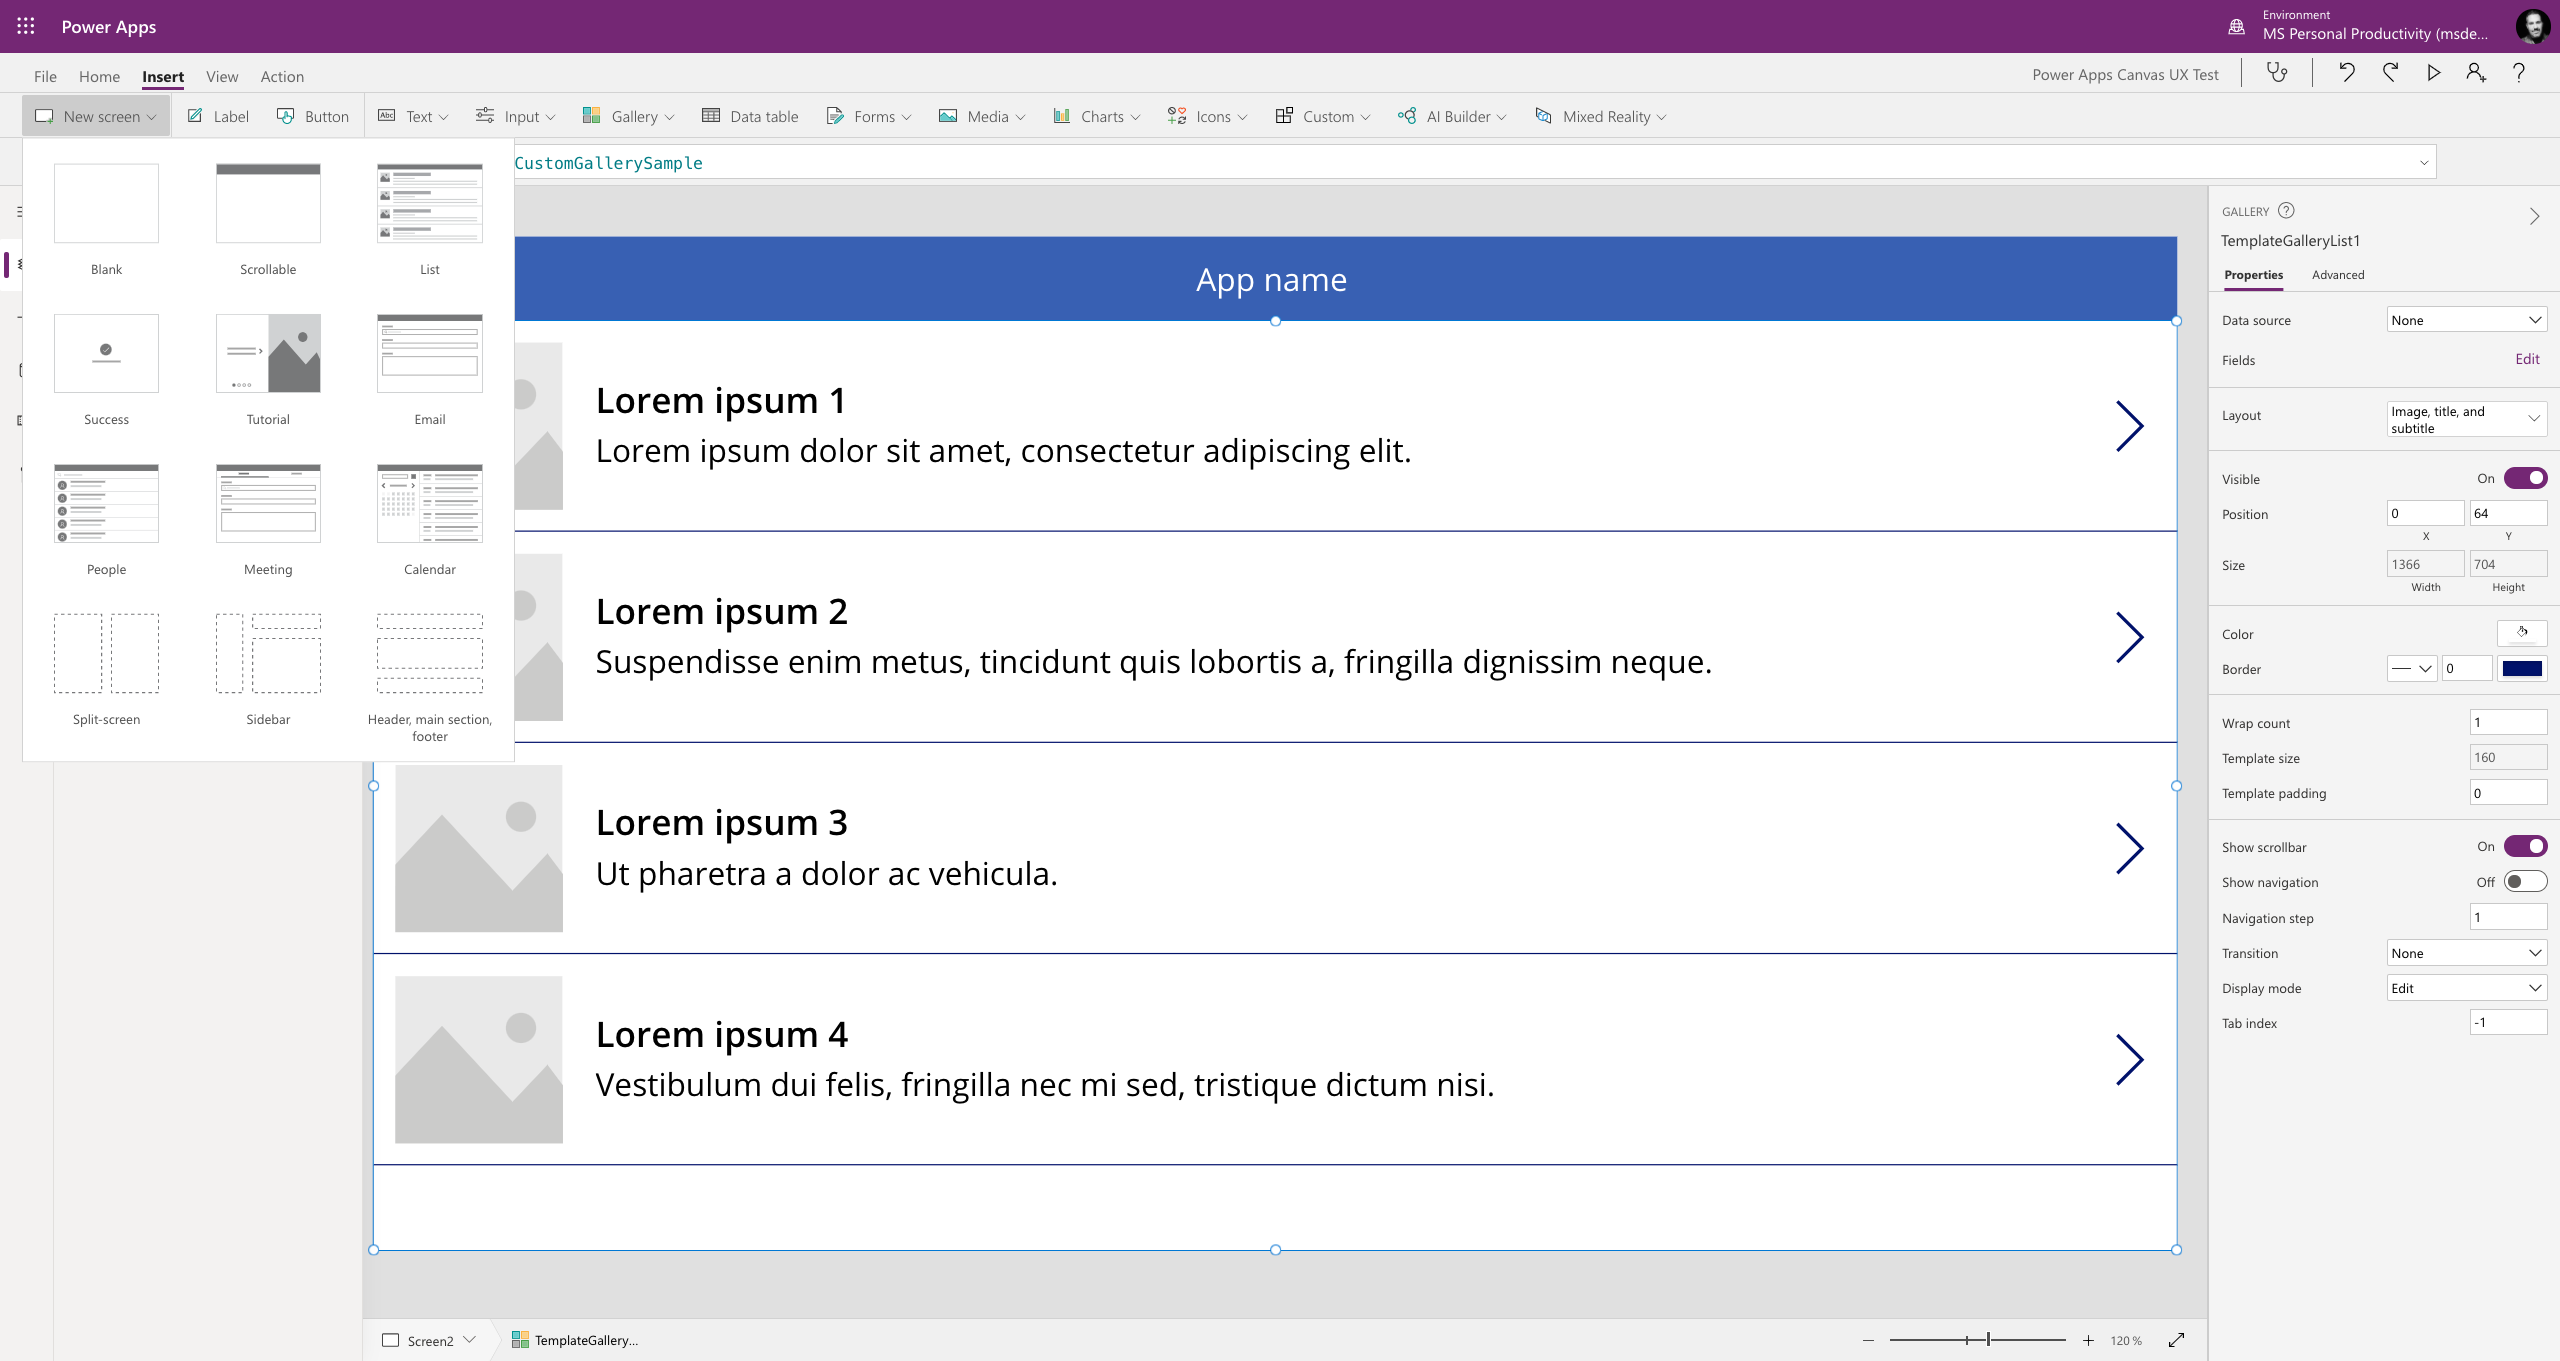
\includegraphics[width=\textwidth]{images/ms_powerapps}
    \captionsource{PowerApps od Microsoft}{\cite{Powerapps2023}}
    \label{fig:pa-plat}
\end{figure}

\vfill
\pagebreak

\begin{figure}[H]
    \centering
    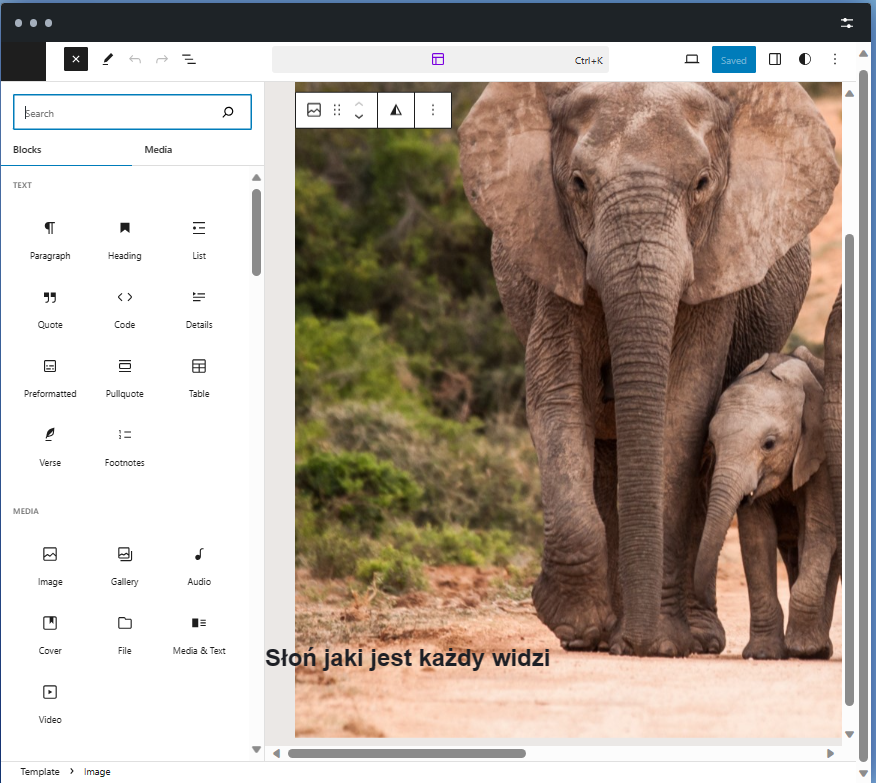
\includegraphics[width=0.8\textwidth]{images/slon_wordpress}
    \captionsource{Wordpress.com}{\cite{WordpressDeveloper2023}}
    \label{fig:wp-plat}
\end{figure}

Coraz większą popularnością cieszą się platformy low-code \trans{ang. Low-code Development Platforms} (\textbf{LCDPs}) dostarczane między innymi przez Google, Microsoft, Amazon.\ Pozwalają one na tworzenie wysoko skalowalnych rozwiązań przy niewielkim albo i żadnym nakładzie pracy z kodem.\ Ma to umożliwić osobom z niewielkim doświadczeniem w programowaniu, na szybkie wdrożenie oraz tworzenie niezawodnego oprogramowania.\ Twórcy platform oferują również korzystającym, zmniejszenie ilości pracy potrzebnej do wdrożenia albo rozwijania kolejnych funkcjonalności~\cite{Bock2021, Hirzel2022}.

LCDP udostępniane twórcom aplikacji, umożliwiają skalowalność rozwiązań tworzonych na własne potrzeby.\ Dodatkowo są popularne przy tworzeniu aplikacji typu ,,\textit{aplikacja jako usługa}'' \trans{ang. Software-as-a-Service} (SaaS), które opłacane są tylko za stopień ich użycia.\ To podejście w konkretnych sytuacjach może się okazać dużo bardziej opłacalne niż utrzymywanie swoich rozwiązań serwerowych.\ Dzięki takim rozwiązaniom wiele małych firm będzie mogło pozwolić sobie na tworzenie i utrzymywanie dostosowanych rozwiązań opartych o ekosystem \textit{Microsoft365} / \textit{Google Workspace}.



\section{Microsoft PowerApps}
Jest to platforma programistyczna umożliwiająca tworzenie niestandardowych aplikacji dla rozwiązań biznesowych.\ Umożliwia ona tworzenie aplikacji opartych o różnorakie źródła danych.\ Do których należą między innymi: SQL Server, SharePoint, Dynamics 365.\ Dodatkową zaletą tego rozwiązania jest tworzenie aplikacji responsywnych, działających dobrze na wielu rodzajach urządzeń.\ Dodatkowo platforma ta pozwala tworzyć trzy typy aplikacji przy braku konieczności kodowania~\cite{Microsoftc}
\begin{itemize}
    \item \textbf{Kanwa} - jest to typ aplikacji oparty o model danych znajdujący się na przykład w Excelu.\ Aplikację tego typu tworzy się za pomocą przesuwanych kafelek, a proces przypomina po trochu robienie prezentacji przy użyciu aplikacji Powerpoint.\ Umożliwia to pełną dowolność w tworzonym interfejsie graficznym~\cite{Microsoftb}.

    \item \textbf{Oparte na modelu} - w ramach korzystania z usługi \textit{Microsoft Dataverse} można wygenerować aplikacje bazujące na danym modelu danych.\ Dzięki czemu użytkownicy otrzymują produkt ułatwiający im analizę danych~\cite{Microsofta}.

    \item \textbf{Karty} - są to uproszczone aplikacje, które można dodać do usługi Microsoft Teams w określonym biznesowym celu.\ Dużą zaletą tego rozwiązania jest możliwość korzystania ze źródeł danych.\ Rozwiązanie to wprowadza możliwość tworzenia aplikacji o pojedynczej odpowiedzialności biznesowej~\cite{Microsoft}.
\end{itemize}

\section{Amazon QuickSight}
Jest to rozwiązanie firmy Amazon, które umożliwia firmom dostarczanie rozwiązań z zakresu analityki biznesowej \trans{ang. business intelligence} (BI).\ Rozwiązanie to dostarcza interaktywne pulpity korzystające z jednego źródła prawdy.\ Dodatkowo korzystanie z interaktywnych formularzy, raportów oraz zapytań w języku naturalnym pozwala interesariuszom otrzymać możliwość korzystania z jednolitych rozwiązań opartych o różne modele danych~\cite{AmazonQuickSight}.

\section{Google AppSheet}
Platforma AppSheet od firmy Google umożliwia tworzenie aplikacji mobilnych oraz desktopowych bez użycia kodu.\ Firma wskazuje na możliwości integracyjne z różnymi dostawcami danych, do których należą między innymi Microsoft, Dropbox.\ Dodatkowo posiada wbudowaną integrację z aplikacjami Google Workspace, do których należą Gmail, Sheets oraz Spaces.\ Platforma pozwala również na tworzenie automatycznych botów, które wykonują zadania po interakcji z bodźce zewnętrznymi bądź wewnętrznymi.\ Narzędzie pozwala w prosty sposób na tworzenie szybkich rozwiązań biznesowych w ekosystemie firmy Google~\cite{GoogleAppSheet}.

\section{Microsoft Azure}
Platforma została oddana do użytku w 2008 roku jako Windows Azure.\ Usługa ta została zbudowana na modułach Windows NT.\ Platforma została udostępniona komercyjnie po 2010 roku, kiedy to dodano możliwość korzystania z szerszej ilości usług i języków programowania.\ Do usług należało między innymi udostępnienie baz danych Microsoft SQL Server opartych o .NET Framework 4, obsługę aplikacji pisanych w wielu języku (takich jak \textit{C\#}, \textit{Java}, \textit{PHP}), sieć dostarczania zawartości \trans{ang. Content Delivery Network} (CDN).
\\ \\
Następnym krokiem było przemianowanie platformy na Microsoft Azure oraz pójście w kierunku infrastruktury definiowanej jako serwis \trans{ang. Infrastructure-as-a-Service} (\textbf{IaaS}), oraz powolne adoptowanie usług open-source.
\\ \\
W kolejnej generacji Microsoft zaadoptował rozwiązania Big Data do swojej platformy, umożliwiając korzystanie z języka \textit{R}, połączenie do Power BI, a także umożliwienie połączenia do rozwiązań end-to-end.
\\ \\
W czwartej generacji platformy, Microsoft skupił się na rozwiązaniach uczenia maszynowego oraz integracji z bazami danych, dzięki czemu powstało Azure Machine Learning Studio oraz Azure Machine Learning Operations (MLOps).
\\ \\
Obecnie platforma została wzbogacona o Kubernetesa, dzięki czemu konteneryzacja ułatwiła pracę z klastrami wirtualnymi.\ Wirtualne klastry pozwalają na wydajniejszy i wygodniejszy sposób zarządzania aplikacjami i usługami.\ Dodatkowo zostało udostępnione wiele kombinacji usług takich jak: aplikacja jako usługa \trans{ang. Software-as-a-Service} (SaaS), Interfejs jako usługa \trans{ang. Infrastucture-as-a-Service} (IaaS), Platforma jako usługa \trans{ang. Platfrom-as-a-Service} (PaaS).\ Microsoft uzyskał w ten sposób platformę przyjazną użytkownikowi, która umożliwia użytkownikom korzystanie z ponad 200 dostępnych usług.\ Dodatkowo płatność za platformę jest rozliczana tylko za zużytą przestrzeń oraz wykorzystaną moc obliczeniową~\cite{Roosevelt2022, MicrosoftAzurec, Datashift}.

\vfill
\pagebreak

\begin{figure}[H]
    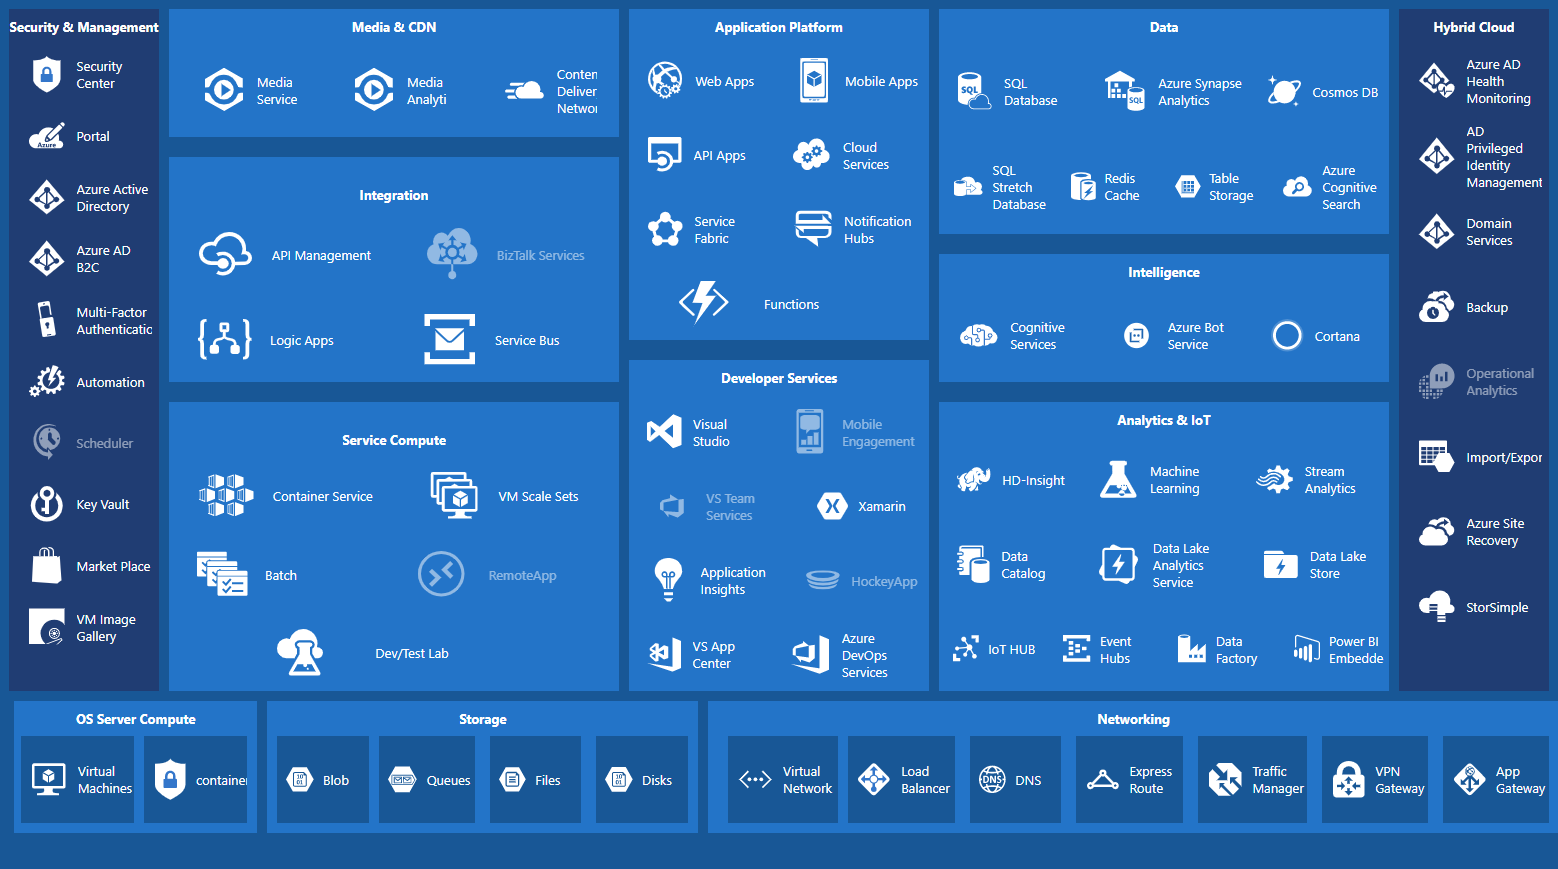
\includegraphics[width=\textwidth]{images/ms_azure}
    \captionsource{Schemat podziału usług MS Azure}{\cite{Datashifta}}
    \label{fig:ms-azure}
\end{figure}

\refsource{Schemat}{fig:ms-azure} pokazuje jak obecnie podzielone są usługi oraz co jest udostępnione komercyjnie w ramach platformy Azure.\ Według schematu platforma podzielona jest na trzynaście obszarów, do których zaliczono między innymi bezpieczeństwo, zarzazanie danymi, usługi deweloperskie, analiza danych, platformy aplikacji.

\section{Infrastruktura}
Infrastruktura globalna Azure składa się z dwóch części: fizycznej infrastruktury oraz globalnej łączności.\ Infrastruktura fizyczna składa się z ponad 200 centrów danych na całym świecie, połączonych w jedną globalną sieć.\ Takie rozwiązanie umożliwia wysoką skalowalność i dostępność poszczególnych rozwiązań.\ Cały ruch sieciowy jest utrzymywany wewnątrz prywatnej sieci Microsoft.\ Pozwala to na zachowanie informacje o adresach IP wewnątrz sieci, a co za tym idzie, informacje te nie trafiają do opinii publicznej~\cite{MicrosoftAzureb}.\\ \\

Na swojej stronie internetowej Microsoft udostępnia wirtualną mapę, umożliwiającą zobaczenie aktualnej sieci Microsoftu oraz jej rozmieszczenie na globie ziemskim.\ Interaktywna mapa pozwala uzyskiwać informację o poszczególnych krajach oraz centrach danych znajdujących się na terytoriach tych krajów.\ Mapę oraz informację pokazano na \refsource{zdjęciach}{fig:azure-ic}.

\vfill
\pagebreak

\begin{figure}[H]
    \begin{subfigure}[m]{0.7\textwidth}
    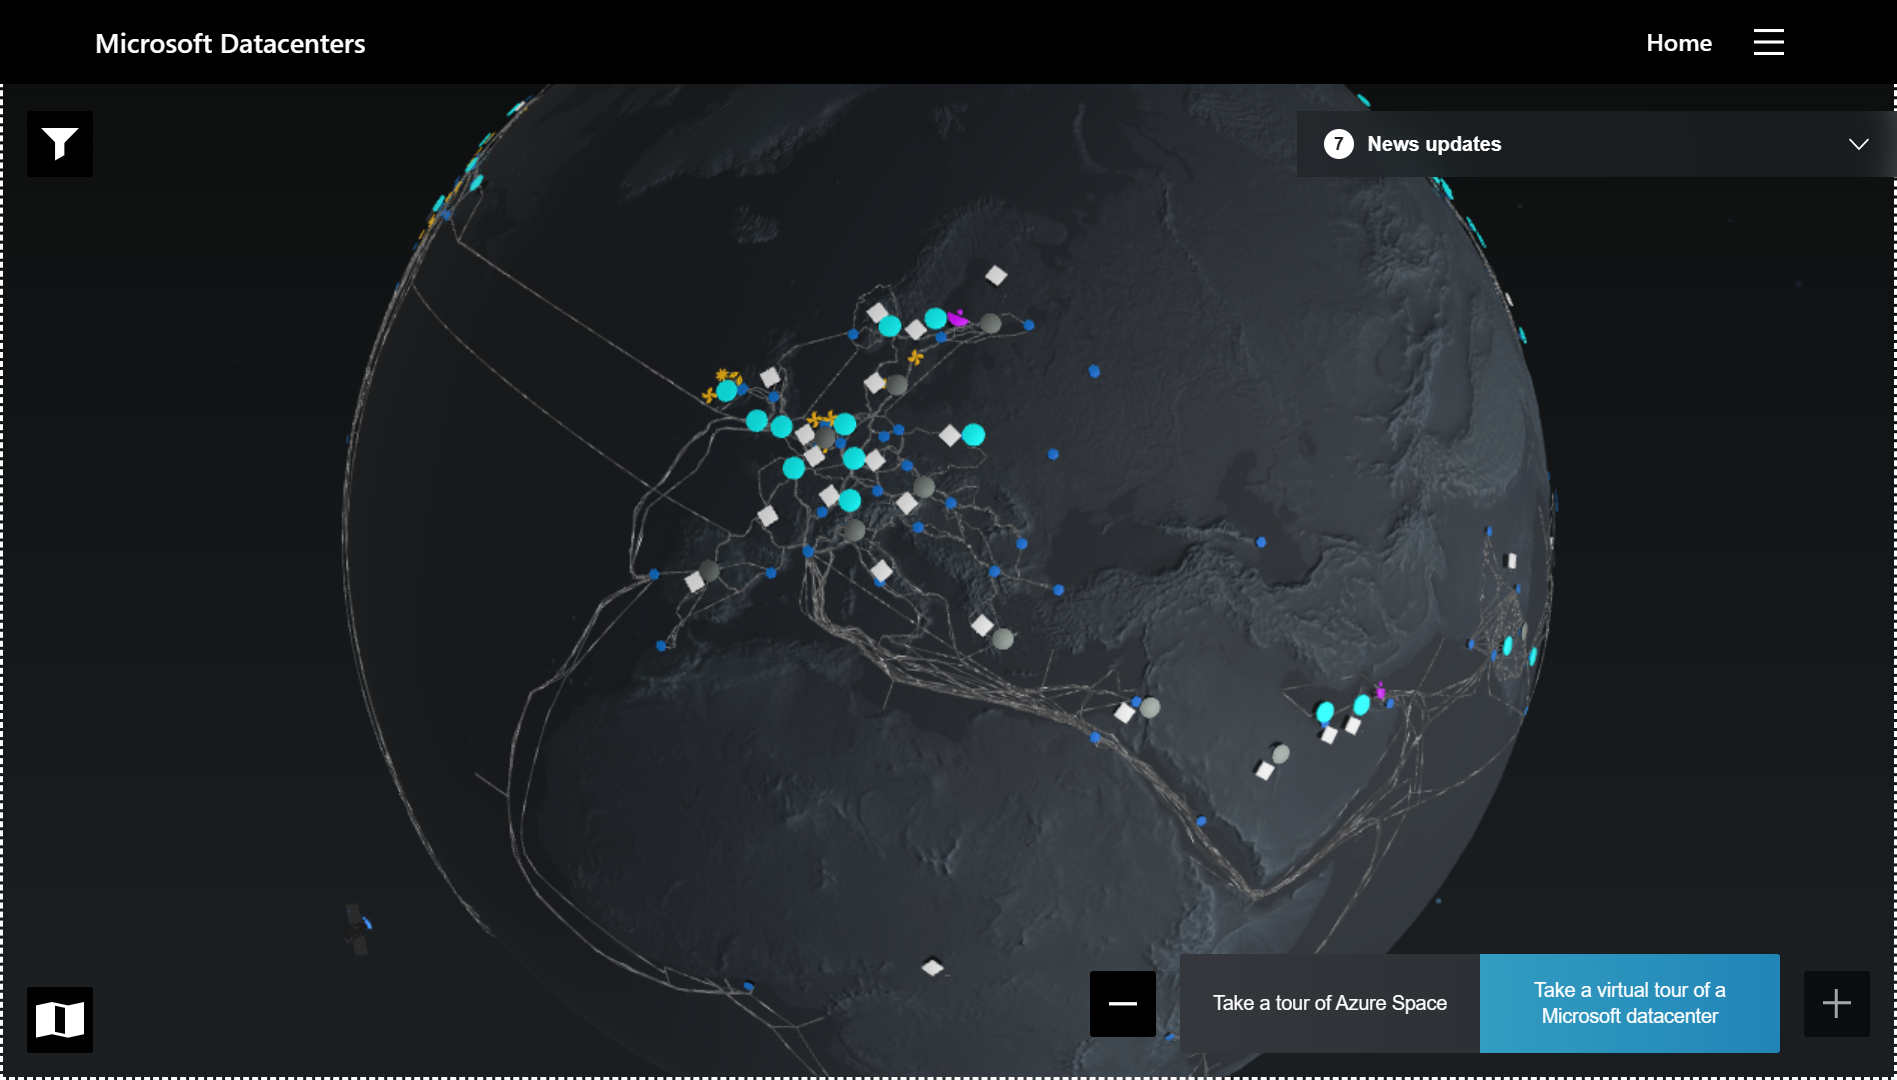
\includegraphics[width=\textwidth]{images/azure-ic}
    \captionsource{Globalna mapa infrastruktury sieciowe}{\cite{MicrosoftAzured}}
    \end{subfigure}
    \hfill
    \begin{subfigure}[m]{0.25\textwidth}
        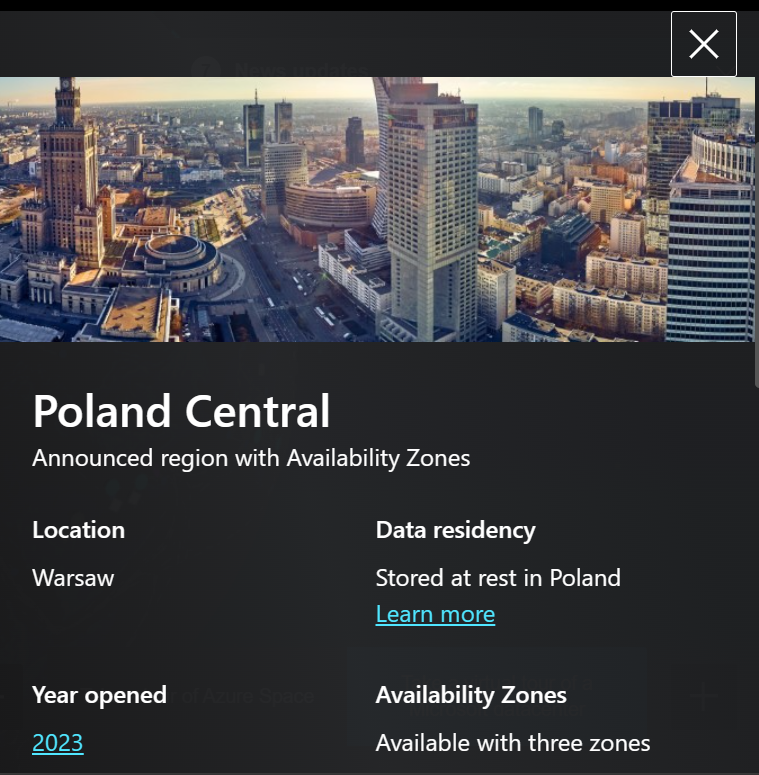
\includegraphics[width=\textwidth]{images/azure-pl}
        \captionsource{Informacje o centrum danych}{\cite{MicrosoftAzuree}}
    \end{subfigure}
    \label{fig:azure-ic}
\end{figure}

\section{Machine Learning Studio}
Azure Machine Learning Studio umożliwia łatwe i szybkie tworzenie wysoce wydajnych modeli uczenia maszynowego, a także zarządzanie nimi.\ Rozwiązanie wspiera pełen cykl życia kompleksowego uczenia maszynowego.\ Platforma umożliwia tworzenie potoków zadań, które połączone w jeden potok, wykonują poszczególne zadania w odpowiedniej kolejności.\ Dzięki modułowej budowie potoków uzyskano rozwiązanie wielokrotnego użytku.\ W ramach jednego doświadczenia każdy moduł może byc buforowany.\ Pozwala to na ,,zapamiętanie'' wyniku poprzedniego uruchomienia i wykorzystanie go ponownie (o ile dane wejściowe albo konfiguracja nie uległy zmianie).\ Dodatkowo poza predefiniowanymi operacjami można wykorzystać moduły języka Python/R.\ Kolejną możliwością jest wytworzenie rozwiązania w technologii ,,\textbf{Jupiter Notebook}'' oraz wizualne narzędzie wykorzystujące mechanizm \textit{przeciągnij i upuść} \trans{ang. Drag \& Drop}.\ Rozwiązanie to pozwala układać ,,\textit{kafelki}'' służące do tworzenia potoków zadań.\ Każde zadanie wykorzystuje wcześniej przygotowaną jednostkę obliczeniową, dzięki czemu można przewidzieć albo dostosować koszt wykorzystania modelu.\ Umożliwione zostało również wdrażanie modeli jako punktów końcowych.\ Pozwala to na komunikowanie się z nimi za pomocą REST API.\\ \\

Microsoft umożliwia płatność jedynie za użytkowanie usług, co oznacza, że jeśli klaster komputerowy był wykorzystywany jedynie przez 1 godzinę, to za tą jedną godzinę zostanie obciążony klient\cite{MicrosoftAzuref}.
